%!TEX ROOT=formularioFisica.tex

\section{Fisica quantistica}
La teoria quantistica nasce nei primi decenni del ventesimo secolo e si pone di studiare problemi
fisici su scala atomica.\\
La fisica quantistica riesce a risolvere il \textbf{problema del corpo nero}.

\subsection{Problema del corpo nero}
Ogni corpo emette radiazioni elettromagnetiche per il movimento delle particelle dovuto alla 
temperatura e ne assorbe alcune. Si definisce $a$ il fattore di assorbimento, $e$ il fattore di 
emissione. Si ha sempre che $0\leq a\leq1$ e $0\leq e\leq1$. Per un corpo nero $a=e=1$.\\
Dato che un corpo così non è realizzabile, si è creato un corpo che si avvicina a queste 
caratteristiche. Esso è schematicametne come il seguente
\begin{center}
  \begin{tikzpicture}
    \draw (0,0) -- (-2,0) -- (-2,3) -- (0,3)  -- (0,1.6) (0,1.4) -- (0,0);
    \draw ($(-0.8,1.5) + (5:0.8)$) arc (5:355:0.8);
    \draw[thick,Dandelion] 
      (1,2) -- ++(210:2.4) -- ++(110:1.2) -- ++(20:1) -- ++(-70:1.2) -- ++(210:0.8) 
      -- ++(50:1.2) -- ++(160:1.3) -- ++(260:1.1);
  \end{tikzpicture}
\end{center}
La caratteristica di questo corpo è di avere una minuscola fessura da cui entra la luce ma non può
uscire. Inoltre è immerso in modo che la temperatura sia costante. Dato che non è un corpo perfetto,
emetterà comunque delle onde elettromagnetiche. Andando a farle passare attraverso un prisma e a
misurare l'intensità di ciascuna lunghezza d'onda si ottiene un grafico di questo tipo
\begin{center}
  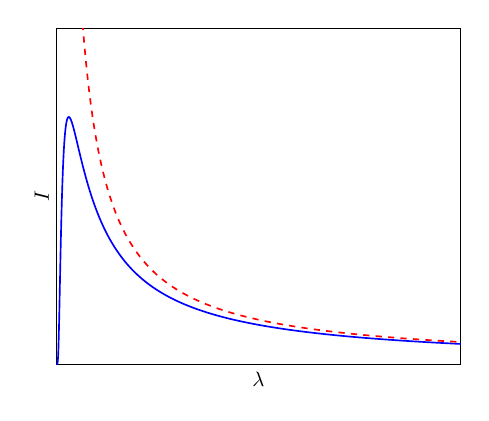
\begin{tikzpicture}[scale=0.75]
    \begin{axis}[xmin=0,ymin=0,xmax=8,ymax=8,xlabel=$\lambda$,ylabel=$I$,ticks=none]
      \addplot[blue,thick,domain=0.01:8,smooth,samples=500] {(4/(e^(1/(4*x))*x))};
      \addplot[red,thick,dashed,domain=0.1:8,smooth,samples=500,unbounded coords=jump]{(7/(e^(1/2)*x))};
    \end{axis}
  \end{tikzpicture}
\end{center}
Questo grafico è stato studiato in moltissim modi e per $lambda$ molto piccoli non si riusciva a
descrivere. L'intensità era definita attraverso la \textbf{legge di Stefan}
\begin{equation*}
  I = \sigma T^4
\end{equation*}
dove $\sigma$ è la \hyperref[tab:sigma]{costante di Stefan-Boltzman}. Si ha inoltre che
\begin{equation*}
  \lambda_{\text{max}}\cdot T=2.9\cdot10^{-3}\,\text{mK}
\end{equation*}
Trovò l'anello mancante lo scienziato tedesco Max Planck. Si arriva finalmente a dimostrare una 
formula, la formula di \textbf{Rayleigh-Jeans}.
\begin{equation*}
  I(\lambda,T) = \frac{2\pi c^2}{\lambda^5} \frac{nh}{e^{\frac{hc}{\lambda k_B T}}-1}
\end{equation*}
$n=1,2,3,\ldots$\\
\hyperref[tab:h]{$h$}: $6.62\cdot10^{-34}\,\text{Js}$\\
\hyperref[tab:c]{$c$}: $3\cdot10^8\,\text{m/s}$\\
\hyperref[tab:kB]{$k_B$}: $1.381\cdot10^{-23}\,\text{J/K}$\\
$T$: temperatura\\
$\lambda$: lunghezza d'onda\\ [\baselineskip]
Questa formula è stata creata anche grazie a alla quantizzazione dell'energia, ovvero
\begin{equation*}
  E = nhf
\end{equation*}
e questo porta alla creazione di un'energia discreta, ovvero che si diffonde non più in modo uniforme
su tutto il fronte d'onda, bensì in pacchetti, denominati quanti.

\subsection{Effetto fotoelettrico}
L'effetto fotoelettrico è valso ad Einstein il Nobel per la Fisica.\\
Il problema era che quando un metallo veniva colpito da un raggio luminoso, alcuni elettroni uscivano
dal corpo. Einstein parte dalla quantizzazione dell'energia.\\
Si definiva \textbf{lavoro di estrazione} il lavoro necessario a strappare l'elettrone dal corpo. 
Quest'ultimo è tenuto legato al corpo dalla \textbf{barriera di potenziale}. Il lavoro qundi diventa
\begin{equation*}
  L = q\Delta V = e\Delta V
\end{equation*}
Considerata che la carica di un elettrone è infinitesimale, si introduce una nuova unità di misura,
l'\textbf{elettron-volt} che è l'energia che acquista un elettrone spostato da $1$V.
\begin{equation*}
  1\,\text{eV} = 1.62\cdot10^{-19}\,\text{J}
\end{equation*}
L'esperimento parte da un oggetto come questo
\begin{center}
  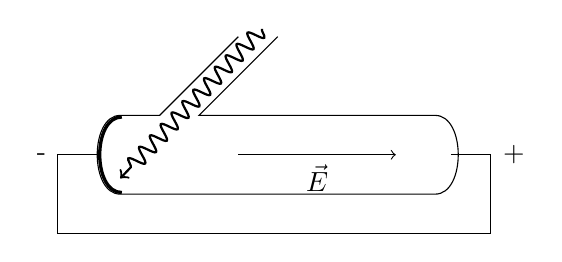
\begin{tikzpicture}[%
    wave/.style={%
        decorate,decoration={snake,post length=1.4mm,amplitude=1mm,
        segment length=2mm},thick},
    ]
    \draw (0,0) to[out=180,in=180] (0,-1) -- (4,-1) to[out=0,in=0] (4,0) -- (1,0) -- (2,1)
      (1.5,1) -- (0.5,0) -- (0,0);
    \draw[very thick] (0.02,-0.02) to[out=180,in=180] (0.02,-0.98);
    \draw[->, wave, thick] (1.8,1.1) -- (0,-0.8);
    \draw (4.2,-0.5) -- ++(0.5,0) -- ++(0,-1) -- ++(-5.5,0) -- ++(0,1) -- ++(0.5,0);
    \node at (-1,-0.5) {-};
    \node at (5,-0.5) {+};
    \draw[->] (1.5,-0.5) -- ++(2,0)
      node[pos=0.5,below]{$\vec{E}$};
  \end{tikzpicture}
\end{center}
Viene fatta passare una radiazione attraverso il tubo apposito, questa va a colpire una lastra di
metallo da cui uscirà un elettrone che, attraverso il campo elettrico, verrà a colpire l'anodo e 
quindi creare una differenza di potenziale. Si ha che se $f$ della radiazione è troppo bassa non si 
avrà effetto. Si ha quindi che
\begin{equation*}
  \Delta V = V_+-V_- = V
\end{equation*}
Il grafico che mette in relazione il potenziale e la corrente è il seguente
\begin{center}
  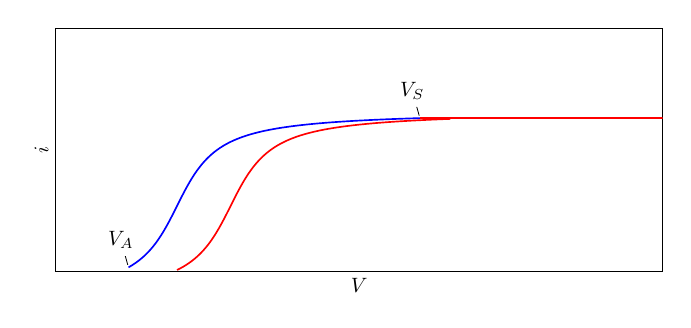
\begin{tikzpicture}[every pin edge/.style={black,thin}, pin distance=7mm,scale=0.75]
    \begin{axis}[xmin=-2,ymin=0,xmax=8,ymax=4,axis equal image,scale=1.5,
      clip mode=individual,xlabel=$V$,ylabel=$i$,ticks=none]
      \addplot[red,thick,smooth,domain=0:4.5,samples=500] {rad(atan(2*x-pi/1.78))+pi/2-0.5};
      \addplot[blue,thick,smooth,domain=-0.8:4,samples=500] {rad(atan(2*x))+pi/2-0.5} 
        coordinate[pos=0] (Va)
        coordinate[pos=1] (Vs);
      \addplot[red,thick,smooth,domain=4:8] {rad(atan(4))+pi/2-0.38};
      \node[inner sep=1pt, pin={[anchor=north]100:$V_A$}] at (Va) {};
      \node[inner sep=1pt, pin={[anchor=north]100:$V_S$}] at (Vs) {};
    \end{axis}
  \end{tikzpicture}
\end{center}
Il grafico in rosso indica quello che accade quando si aumenta $V$, in blu invece quando si torna
ad abbassare.\\
I punti segnati sono rispettivamente il \textbf{potenziale di arresto} ($V_A$) ovvero la frequenza
in cui non si genera corrente e \textbf{potenziale di saturazione} ($V_S$).\\
Sapendo che
\begin{equation*}
  L = eV_A = E_c
\end{equation*}
è possibile calcolare l'energia ginetica dell'elettrone. Sapendo che
\begin{equation*}
  E=hf
\end{equation*}
e che il fotone deve vincere il lavoro di estrazione e l'energia cinetica dell'elettrone, si può
scrivere per la legge della conservazione dell'energia
\begin{equation*}
  hf=eV+E_c \rightarrow E_c=hf-eV
\end{equation*}
Si noti che se $E_c=0$, si trova la frequenza di soglia, ovvero
\begin{equation*}
  f_s = \frac{eV}{h}
\end{equation*}

\subsection{Effetto Compton}
L'effetto Compton viene scoperto studiando l'effetto fotoelettrico in cui un elettrone e un fotone
si scontrano.
\begin{center}
  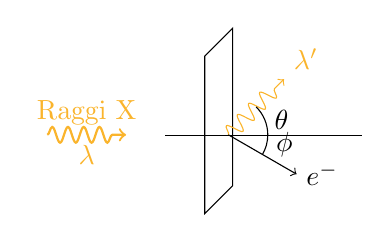
\begin{tikzpicture}[%
    wave/.style={%
        decorate,decoration={snake,post length=1.4mm,amplitude=1mm,
        segment length=2mm},thick},
    ]
    \draw[wave,->,Dandelion] (0,0) -- (1,0)
      node[pos=0.5,above]{Raggi X}
      node[pos=0.5,below]{$\lambda$};
    \draw[very thin] (1.5,0) -- (4,0);
    \draw (2,1) -- ++(45:0.5) -- ++(-90:2) -- ++(225:0.5) -- cycle;
    \draw[wave,->,thin,Dandelion] (2.3,0) -- ++(45:1) 
      node[pos=1,above right] {$\lambda'$};
    \draw[->,thin] (2.3,0) -- ++(-30:1)
      node[pos=1,right] {$e^-$};
    \draw (2.8,0) arc (0:45:0.5)
      node[pos=0.5,right]{$\theta$};
    \draw (2.8,0) arc (0:-30:0.5)
      node[pos=0.5,right]{$\phi$};
  \end{tikzpicture}
\end{center}
Questo viene considerato un urto elastico tra particelle, quindi $E_c$ si conserva. La quantità di 
moto ha modulo
\begin{equation*}
  q = \frac{E}{c}= \frac{hf}{c} = \frac{h}{\lambda}
\end{equation*}
Prima dell'urto, l'elettrone è fermo, quindi si ha soltanto l'energia del fotone. Dopo si può 
scrivere il seguente sistema
\begin{equation*}
  \begin{cases}
    \frac{hc}{\lambda}=\frac{hc}{\lambda'} + \overbrace{mc^2(\gamma-1)}^{E_c}\\
    \frac{h}{\lambda}=\frac{h}{\lambda'}\cos\theta+mv\gamma\cos\phi\\
    0=\frac{h}{\lambda'}\sin\theta+mv\gamma\sin\phi
  \end{cases}
\end{equation*}
La prima equazione è per la conservazione dell'energia, le seconde due sono le componenti orizzontali
e verticali della quantità di moto. La soluzione di questo sistema si ottiene nella forma
\begin{equation*}
  \lambda'-\lambda=\frac{h}{mc}(1-\cos\theta)
\end{equation*}
da cui si evince che
\begin{equation*}
  \lambda'>\lambda \rightarrow f'<f \rightarrow \text{Perde energia}
\end{equation*}

\subsection{Spettrometria}
Si è visto che gli atomi emettono fotoni facendo passare il raggio attraverso un prisma, si ottengono
delle serie spettrali. Le tre serie principali sono
\begin{description}
  \item[Balmer] Serie del visibile
  \item[Lyman] Serie dell'ultravioletto
  \item[Paschen] Serie dell'infrarosso
\end{description}
Si è notato che se la sostanza aeriforme è eccitata sempre allo stesso modo, si ottiene sempre la
stessa serie.
\begin{center}
  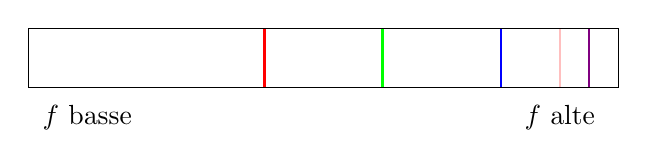
\begin{tikzpicture}[scale=0.75]
    \draw[thick,red](4,0)-- (4,1);
    \draw[thick,green](6,0)-- (6,1);
    \draw[thick,blue](8,0)-- (8,1);
    \draw[thick,pink](9,0)-- (9,1);
    \draw[thick,violet](9.5,0)-- (9.5,1);
    \draw (0,0)--(10,0)--(10,1)--(0,1)--(0,0);
    \node at (1,-0.5) {$f$ basse};
    \node at (9,-.5) {$f$ alte};
  \end{tikzpicture}
\end{center}
Balmer ha trovato una formula sperimentale per identificare la lunghezza d'onda della $n$-esima 
frangia
\begin{equation*}
  \lambda_n = 364.6 \frac{n^2}{n^2-4}\quad n\geq3
\end{equation*}
Qualche tempo dopo Rydberg è riuscito a generalizzare la formula
\begin{equation*}
  \frac{1}{\lambda}=R \left( \frac{1}{n^2_f}-\frac{1}{n^2_i} \right)
\end{equation*}
dove $R=10.79\,\mu\text{m}$ è una costante.\\
È da notare che queste serie sono particolari per alcuni particolari valori di $n$, la formula di
Rydberg è generale. È inoltre impotante notare che \textbf{l'atomo in questione è sempre quello di
idrogeno}.

\subsection{Modelli atomici}
Con le nuove scoperte e le nuove informazioni, si è cercato di creare dei sistemi atomici che 
spiegassero le esperienze fatte.
\subsubsection{Atomo di Thompson}
L'atomo di Thompson (comunemente detto ``a panettone'') era un atomo in cui gli elettroni si 
muovevano liberamente in uno spazio chiuso. Questo modello entrava in crisi quando si sparavano raggi
$\alpha$ e alcuni di questi raggi tornavano indietro. Non si riusciva a trovare una spiegazione di
questo fatto
\subsubsection{Atomo di Rutherford}
Rutherford riprende un sistema planetario. Dato che la fisica macroscopica era gestita secondo un
sistema planetario come quello di Newton, Rutherford ipotizza che anche l'atomo sia così. Un nucleo
attorno a cui gli elettroni ruotano attorno. Il problema era: l'elettrone è in moto o è fermo?
Non può essere fermo in quanto l'atomo collasserrebbe. Se fosse in moto si muoverebbe di moto 
circolare uniforme, che è un moto accelerato. Dato che evidenze sperimentali mostrano la creazione di
onde elettromagnetiche e dato che l'energia non è infinita, l'elettrone dovrebbe perdere pian piano
energia fino a schiantarsi contro il nucleo.
\subsubsection{Atomo di Bohr}
Bohr si pone come obiettivo quello di spiegare le linee spettrali. Pone come vero che l'elettrone si
muove su alcune orbite e fintanto che è stazionario non irradia energia. Bohr pone due ipotesi 
fondamentali
\begin{enumerate}
  \item L'elettrone è mantenuto sull'orbita per forza coulombiana
  \item Il momento angolare si conserva
\end{enumerate}
Specialmente quest'ultima è innovativa. Infatti Bohr \textbf{quantizza il momento angolare} in modo
che l'espressione diventi
\begin{equation*}
  L = n \frac{h}{2\pi} = n\hbar
\end{equation*}
Bohr ora, per dimostrare che il suo modello funzioni davvero, vuole arrivare alla formula di Rydberg.
\paragraph{Raggi delle orbite degli elettroni}
Bohr parte dalla legge della conservazione dell'energia e utilizza la sua seconda ipotesi per 
scrivere il seguente sistema
\begin{equation*}
  \begin{cases}
    \overbrace{k \frac{e^2}{r^2}}^{\text{Coulomb}}=
    \overbrace{m \frac{v^2}{r}}^{\mathclap{\text{\parbox{4cm}{\centering Accelerazione\\[-4pt]
    Centripeta}}}}\\
    mvr=n \frac{h}{2\pi}
  \end{cases}
\end{equation*}
Che risolto per $r$ ottiene come risultato
\begin{equation*}
  r = \frac{n^2h^2}{4\pi ke^2m} = \frac{h^2}{4\pi \frac{1}{4\pi\varepsilon_0}e^2m}n^2=
  \frac{\varepsilon_0h}{\pi e^2m}n^2 = r_0 n^2
\end{equation*}
\paragraph{Energia dell'elettrone}
Sapendo che l'energia si conserva, Bohr arriva a scrivere
\begin{equation*}
  E = E_c + U = \frac{1}{2}mv^2-k \frac{e^2}{r} = 
  \frac{1}{2}m\overbrace{k\frac{e^2}{r}}^{\mathclap{\text{\parbox{4cm}{\centering Dimostrato \\[-4pt]
  nel raggio}}}}-k \frac{e^2}{r} = -\frac{1}{2}k \frac{e^2}{r}
\end{equation*}
Ora avendo noi trovato l'espressione per il raggio nel paragrafo precedente, sostituiamo.
\begin{equation*}
  E_n=-\frac{1}{2}k \frac{e^2}{r_n}=-\frac{1}{2}\frac{1}{4\pi\varepsilon_0}
  \frac{e^2}{\varepsilon_0h^2}\pi e^2m\frac{1}{n}=
  -\frac{me^4}{8\varepsilon_0^2h^2}\frac{1}{n}= -\frac{E_0}{n}
\end{equation*}
Dove $E_0 = 13.6\,\text{eV}$.\\
\paragraph{Salto quantico}
Andando ad analizzare i valori di $E_n$ per $n\to\infty$, si vede che tendono a $0$. Per l'ipotesi
di Bohr, un elettrone emette energia solo quando salta da un'orbita all'altra. Quindi le serie
di Balmer o simili sono esempi di salto quantico. Bohr arriva a formulare la seguente formula
\begin{equation*}
  hf = \abs{E_i-E_f}
\end{equation*}
che non è altro che la conservazione dell'energia (si noti che in caso di emissione, si tolga il
modulo). Andando a modificare la formula
\begin{equation*}
  hf=-\frac{E_0}{n_i^2}+\frac{E_0}{n_f^2} \rightarrow f = 
  \frac{E_0}{h}\left( \frac{1}{n_f^2}-\frac{1}{n_i^2} \right)
\end{equation*}
Andando a sostituire la frequenza
\begin{equation*}
  \frac{c}{\lambda}=\frac{E_0}{h}\left( \frac{1}{n_f^2}-\frac{1}{n_i^2} \right)
\end{equation*}
E infine
\begin{equation*}
  \frac{1}{\lambda}=\frac{E_0}{ch}\left( \frac{1}{n_f^2}-\frac{1}{n_i^2} \right)
\end{equation*}
Se si dimostra che $E_0/ch = R$ allora significa che il modello di Bohr funziona.
\begin{equation*}
  E_0= \frac{\frac{me^4}{8\varepsilon_0^2h^2}}{ch}= \frac{me^4}{8\varepsilon_0^2h^3c}=R
\end{equation*}
Questo dimostra che l'atomo di Bohr, semi-quantistico, funziona per l'atomo di idrogeno. Si noti che
le serie si ottengono
\begin{description}
  \item[per $n_f=1$] di Lyman
  \item[per $n_f=2$] di Balmer
  \item[per $n_f=3$] di Paschen
\end{description}
\paragraph{Disegno di atomo}
\begin{center}
  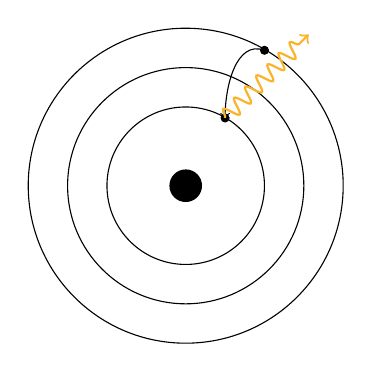
\begin{tikzpicture}[wave/.style={%
      decorate,decoration={%
        snake,post length=1.4mm,amplitude=1mm,
        segment length=2mm
      },thick
    },
    ]
    \draw (0,0); 
    \draw (0,0) circle (1);
    \draw (0,0) circle (1.5);
    \draw (0,0) circle (2);
    \filldraw (0,0) circle (0.2);
    \filldraw (1,0.86*2) circle (0.05);
    \draw[->] (1,0.86*2) to[out=160,in=90] (0.5,0.86);
    \filldraw (0.5,0.86) circle (0.05);
    \draw[wave,->,Dandelion] (0.5,0.86) -- +(45:1.5);
  \end{tikzpicture}
\end{center}
